\documentclass[UTF8, a4paper, 11pt]{ctexart}
\usepackage{geometry}
\usepackage{graphicx}
\usepackage{float}
\usepackage{listings}
\usepackage{xcolor}
\usepackage{hyperref}

% 设置页边距
\geometry{left=2.5cm, right=2.5cm, top=2.5cm, bottom=2.5cm}

% 定义代码块的显示格式（移除危险的转义符，保证代码块绝对安全）
\lstset{
    language=Matlab,
    backgroundcolor=\color{gray!10},
    frame=single,
    keywordstyle=\color{blue},
    commentstyle=\color{gray},
    basicstyle=\ttfamily\small,
    breaklines=true
}
\usepackage[UTF8]{ctex} % 支持中文
\usepackage{geometry} % 页面边距设置
\geometry{left=2.5cm, right=2.5cm, top=3cm, bottom=3cm}
\usepackage{graphicx} % 插入图片
\usepackage{float} % 图片位置控制
\usepackage{caption} % 图片标题
\usepackage{subcaption} % 子图
\usepackage{color} % 颜色
\usepackage{booktabs} % 三线表
\usepackage{hyperref} % 超链接
\usepackage{fancyhdr} % 页眉页脚
\usepackage{amsmath}
% 设置超链接样式
\hypersetup{
    colorlinks=true,
    linkcolor=blue,
    filecolor=magenta,      
    urlcolor=cyan,
}

% 页眉页脚设置
\pagestyle{fancy}
\fancyhf{}
\fancyhead[L]{西湖水图像处理工具}
\fancyhead[R]{课程设计报告}
\fancyfoot[C]{\thepage}

\usepackage{listings}
\usepackage{xcolor}

\definecolor{codegreen}{rgb}{0,0.6,0}
\definecolor{codegray}{rgb}{0.5,0.5,0.5}
\definecolor{codepurple}{rgb}{0.58,0,0.82}
\definecolor{backcolour}{rgb}{0.95,0.95,0.92}

\lstset{
    backgroundcolor=\color{backcolour},   
    commentstyle=\color{codegreen}\itshape,
    keywordstyle=\color{blue}\bfseries,
    numberstyle=\tiny\color{codegray},
    stringstyle=\color{codepurple},
    basicstyle=\ttfamily\footnotesize,
    breakatwhitespace=false,         
    breaklines=true,                 
    captionpos=b,                    
    keepspaces=true,                 
    numbers=left,                    
    numbersep=5pt,                  
    showspaces=false,                
    showstringspaces=false,
    showtabs=false,                  
    tabsize=2,
    frame=single,
    frameround=tttt,
    rulecolor=\color{black!30}
}
\setlength{\headheight}{15pt}
\begin{document}
\begin{titlepage}
    \begin{center}
        \vspace*{2cm}
        \Huge{\textbf{基于 MATLAB App Designer 的交互式图像分析系统设计}}\\
        \vspace{0.5cm}
        \Large{\textbf{——西湖水图像处理系统}}\\
        \vspace{2cm}
        
        \large
        \begin{tabular}{rl}
            \textbf{学生姓名：} & [姓名] \\  % <--- 这里改成你的名字
            \textbf{学号：} & [学号] \\      % <--- 这里改成你的学号
            \textbf{完成日期：} & \today \\
        \end{tabular}
        \vspace{3cm}
        
        \rule{0.8\textwidth}{0.5pt} \\
        \vspace{0.5cm}
        \textit{我设计并实现了一个基于 MATLAB App Designer 的交互式图像处理与特征分析 App。本 App 实现了图像增强、Canny 边缘提取，以及图像灰度 3D 拓扑图的实时渲染。}
    \end{center}
\end{titlepage}

\newpage
\newpage

\section{选题背景与设计目标}
本课程设计围绕专业课中信号与系统以及数字信号处理相关理论展开。在专业课中，图像通常被视为二维离散信号。为了更直观地理解图像的时频域变换、空间边缘提取以及区域特征分析，我设计并开发了这款基于 MATLAB App Designer 的交互式图像分析系统。


本设计的目标是实现一个功能完整的图像处理软件，具备以下核心能力：
\begin{enumerate}
    \item 支持图像的导入、自适应增强、伪彩色映射及导出。
    \item 结合频域分析理论实现二维快速傅里叶变换的可视化。
    \item 实现鼠标拖拽区域的实时截图与边缘轮廓同步提取。
    \item 重构图像空间灰度分布，生成可3D旋转的亮度拓扑图。
\end{enumerate}

section{系统总体设计与界面布局}
为保障软件的易用性，我采用了单窗多选项卡的布局结构。

系统主要分为三个功能选项卡：
\begin{itemize}
    \item \textbf{智能增强与频域分析：} 负责基础图像文件的导入导出并 CLAHE 增强。
    \item \textbf{交互式智能分割：} 提供鼠标手绘框选区域的功能，右侧小窗口会实时动态显示框选区域的轮廓提取结果。
    \item \textbf{3D特征映射可视化：} 将二维图像转换为三维空间地貌图，支持用鼠标在画板上进行任意视角的旋转和缩放。
\end{itemize}

% 截图位置 1：软件整体界面布局
\begin{figure}[H]
    \centering
    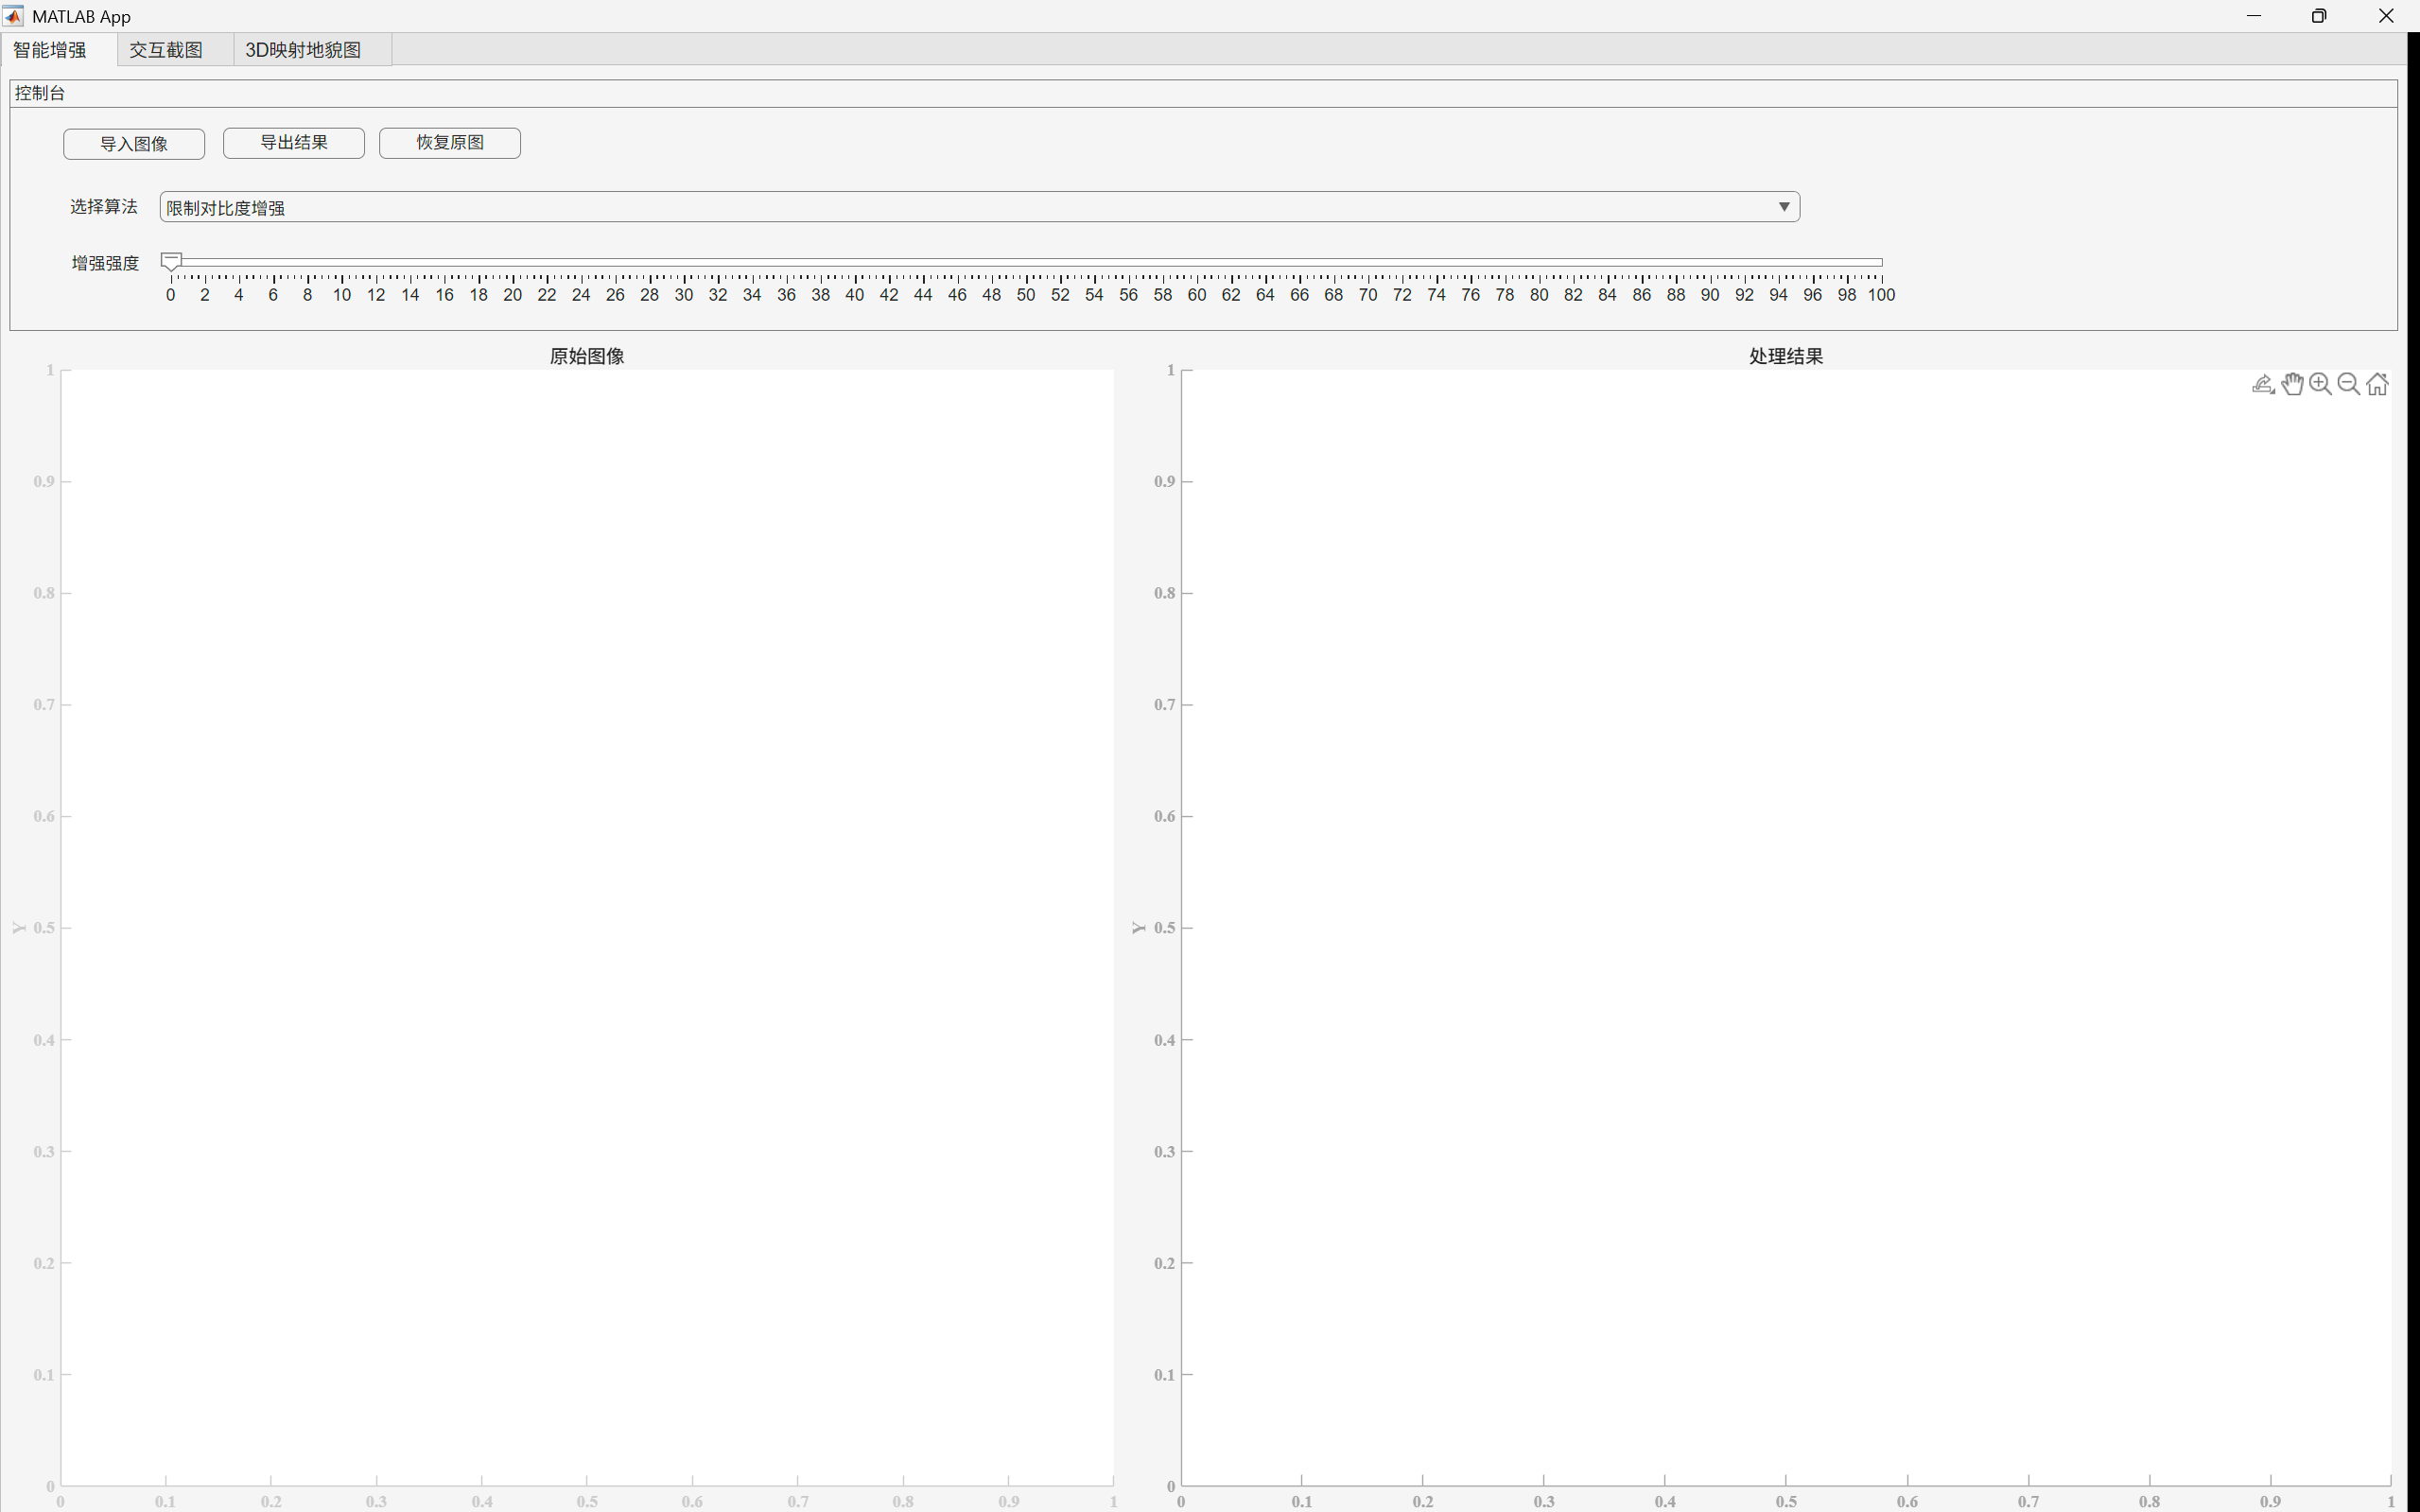
\includegraphics[width=0.85\textwidth]{ui_main.png}
    \caption{主界面示意图}
    \label{fig:ui_main}
\end{figure}

\section{核心功能与关键代码实现}

\subsection{全局变量与数据管理}
在 App 后台，我定义了私有属性来存储原始图像和当前处理的图像矩阵。这种设计避免了使用全局变量引起的命名冲突，保证了数据在不同选项卡和按钮回调之间的安全传递。

\begin{lstlisting}
properties (Access = private)
    ImgOriginal % 存储读入的原始图像数据
    ImgCurrent  % 存储当前算法处理后的图像数据
end
\end{lstlisting}

\subsection{算法动态参数调节}
为了实现人机交互的实时性，我将滑块与算法参数进行了绑定。当用户拖动滑块时，程序会读取数值并动态计算。以下是滑块数值改变时的核心控制代码：

\begin{lstlisting}
% 滑块数值改变回调函数
function Slider_IntensityValueChanged(app, event)
    if isempty(app.ImgOriginal), return; end
    sliderVal = app.Slider_Intensity.Value; 
    selectedAlgo = app.Drop_Algo.Value;     
    
    switch selectedAlgo
        case 'CLAHE限制对比度增强'
            clipLimitValue = 0.01 + (sliderVal / 100) * 0.19; 
            if size(app.ImgOriginal, 3) == 3
                labImg = rgb2lab(app.ImgOriginal);
                L = labImg(:,:,1) / 100;
                L_enhanced = adapthisteq(L, 'NumTiles', [4 4], 'ClipLimit', clipLimitValue);
                labImg(:,:,1) = L_enhanced * 100;
                app.ImgCurrent = lab2rgb(labImg);
            else
                app.ImgCurrent = adapthisteq(app.ImgOriginal, 'NumTiles', [4 4], 'ClipLimit', clipLimitValue);
            end
            
        case '边缘提取'
            thresh = 0.1 + ((100 - sliderVal) / 100) * 0.7; 
            if size(app.ImgOriginal, 3) == 3
                grayImg = rgb2gray(app.ImgOriginal);
            else
                grayImg = app.ImgOriginal;
            end
            edgeImg = edge(grayImg, 'Canny', thresh);
            app.ImgCurrent = uint8(edgeImg) * 255;
    end
    imshow(app.ImgCurrent, 'Parent', app.UIAxes_Result); 
end
\end{lstlisting}

% 截图位置 2：算法处理效果对比（例如边缘提取或CLAHE增强）
\begin{figure}[H]
    \centering
   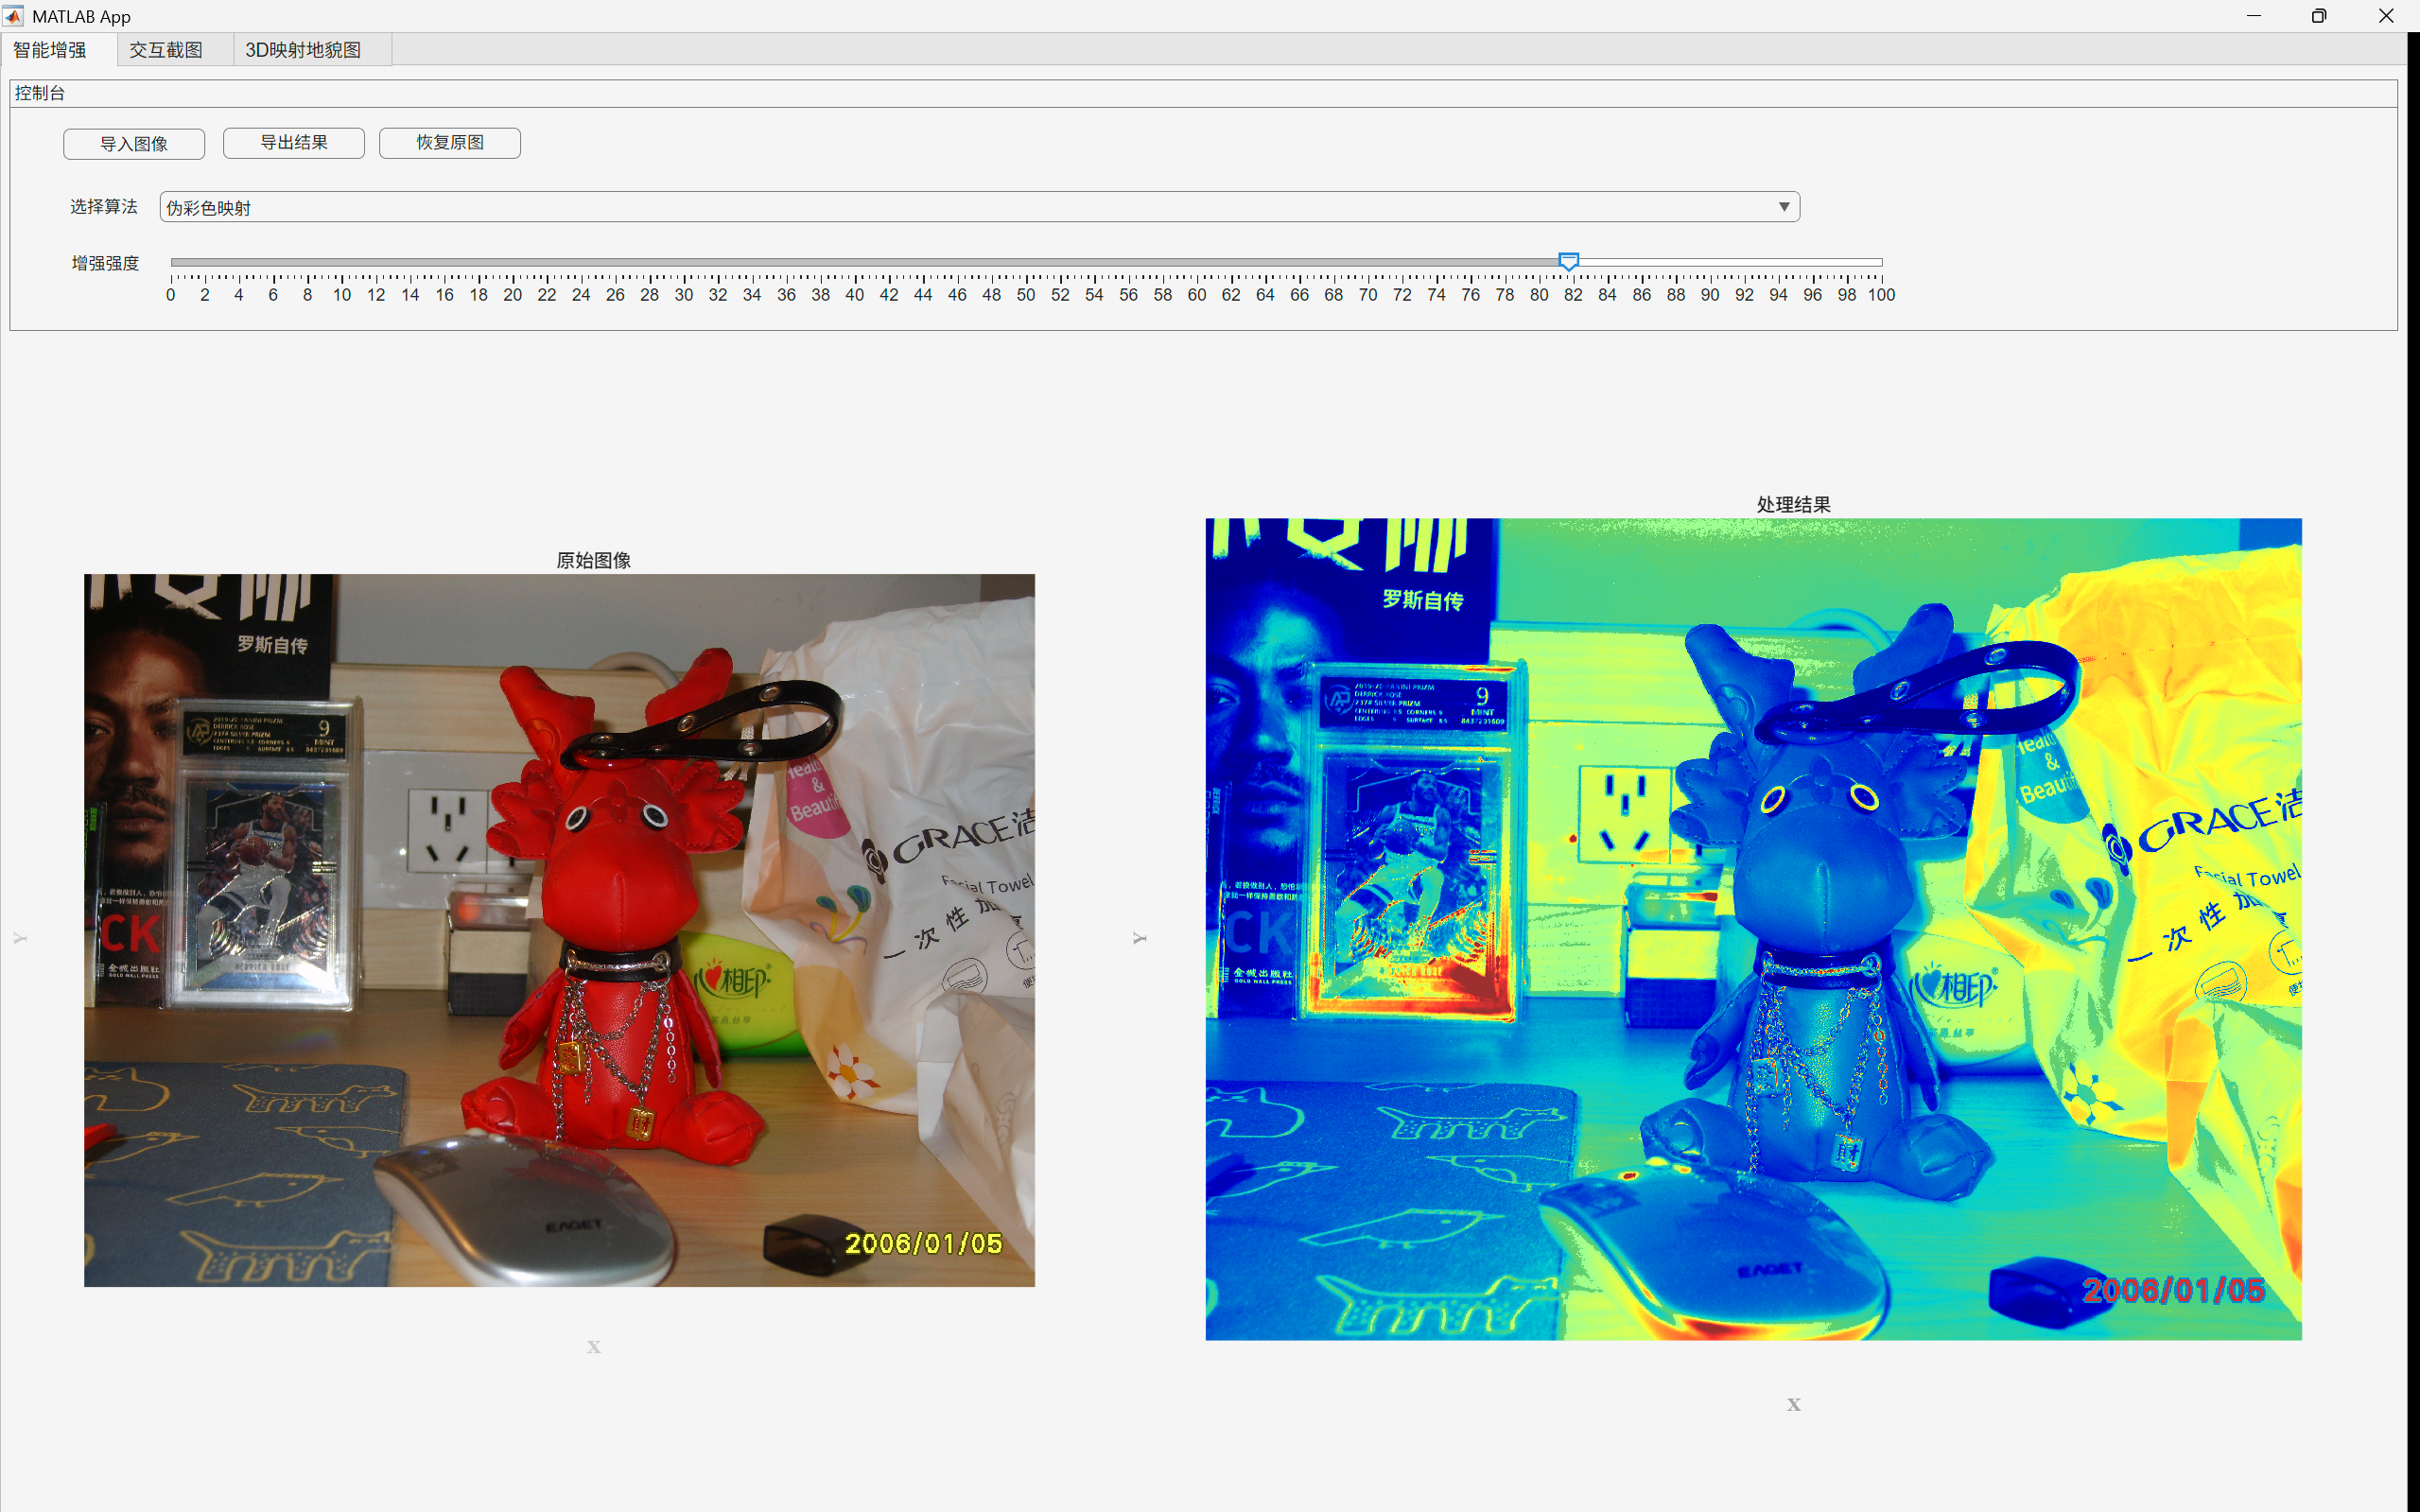
\includegraphics[width=0.85\textwidth]{algorithm_result.png}
    \caption{图像处理算法前后对比效果}
    \label{fig:algorithm}
\end{figure}

\subsection{基于事件监听的实时 ROI 截图}
在第二个选项卡中实现了鼠标拖拽红框右侧小图跟着实时刷新的动态效果，我没有采用静态单次截图的做法，而是引入了事件监听机制，将红框的拖动事件与后台函数绑定。

\begin{lstlisting}
function Btn_ROIPushed(app, event)
    if isempty(app.ImgOriginal), return; end
    disableDefaultInteractivity(app.UIAxes_SegMain);
    imshow(app.ImgOriginal, 'Parent', app.UIAxes_SegMain);
    
    try
        roi = drawrectangle(app.UIAxes_SegMain, 'Label', '目标提取区', 'Color', 'r', 'LineWidth', 2);
        app.processAndShowCrop(roi.Position);
        addlistener(roi, 'MovingROI', @(src, event) app.processAndShowCrop(event.CurrentPosition));
    catch 
        disp('用户取消了操作');
    end
end
\end{lstlisting}

% 截图位置 3：手绘ROI实时联动效果
\begin{figure}[H]
    \centering
    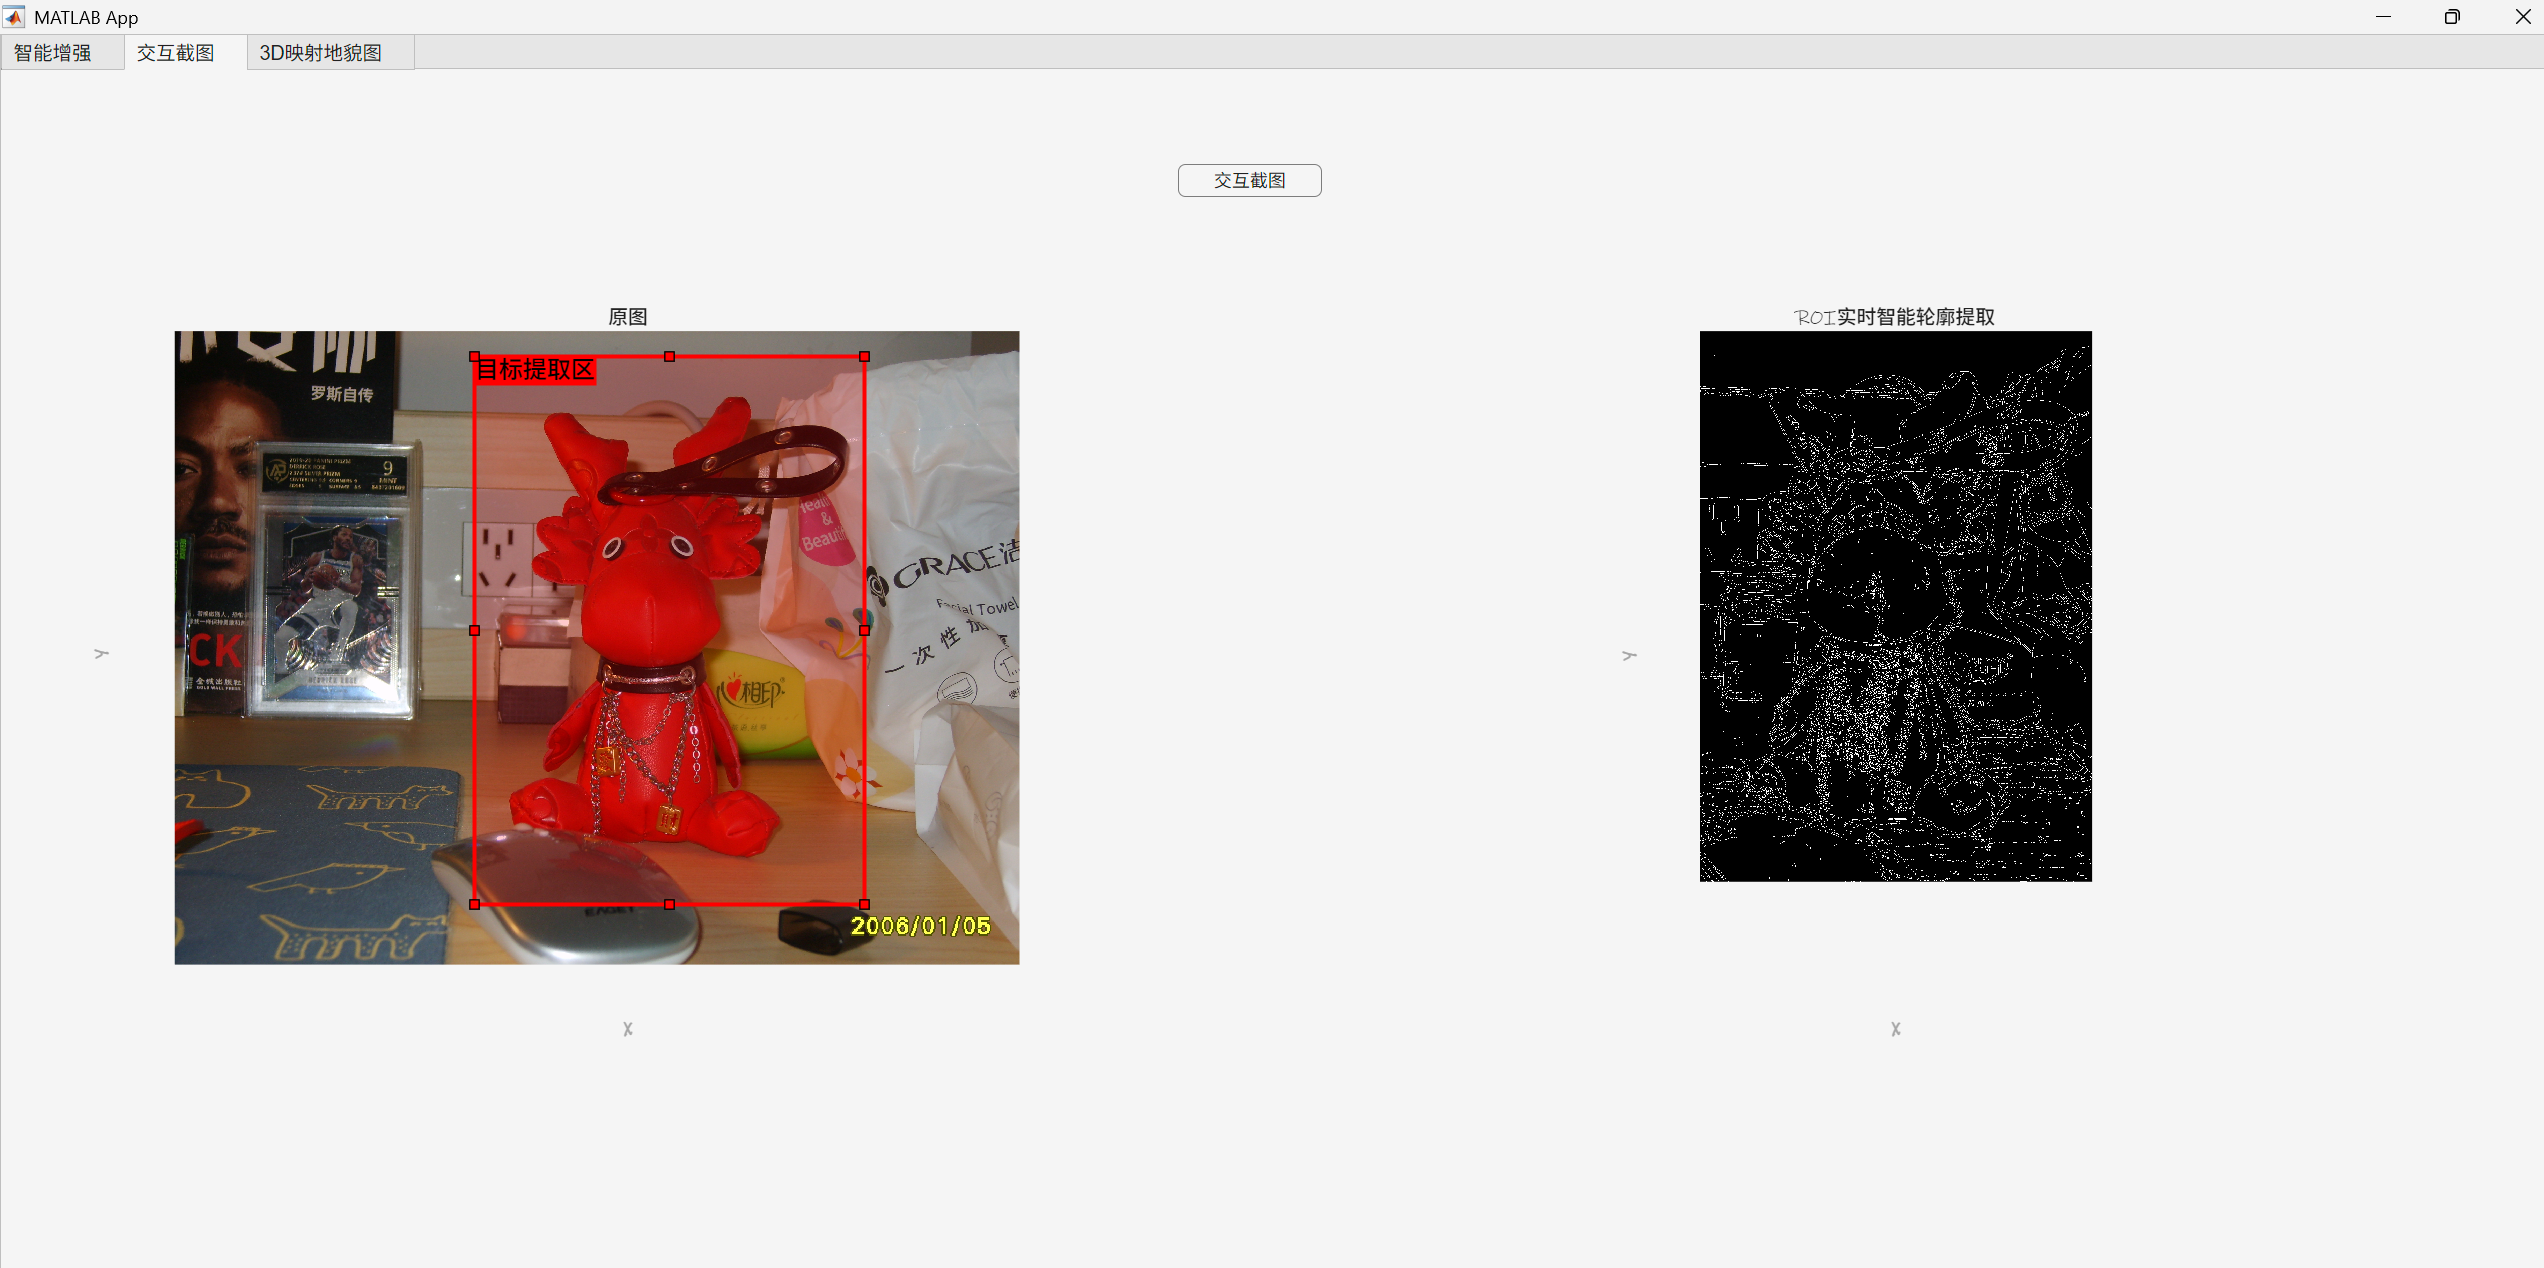
\includegraphics[width=0.85\textwidth]{roi_live.png}
    \caption{实时截图界面}
    \label{fig:roi}
\end{figure}

\subsection{二维图像的3D亮度地貌重构}
第三个选项卡将二维矩阵转换为三维空间网络。代码通过降低分辨率并调用 \texttt{surf} 函数，绘制出图像灰度值的拓扑波动图。

\begin{lstlisting}
function Btn_3DPushed(app, event)
    if isempty(app.ImgOriginal), return; end
    if size(app.ImgOriginal, 3) == 3
        grayImg = rgb2gray(app.ImgOriginal);
    else
        grayImg = app.ImgOriginal;
    end
    smallImg = imresize(grayImg, [200, 200]); 
    
    % 绘制三维表面图
    surf(app.UIAxes_3D, double(smallImg), 'EdgeColor', 'none');
    colormap(app.UIAxes_3D, 'parula');
    view(app.UIAxes_3D, -37.5, 30); 
    grid(app.UIAxes_3D, 'on');
    enableDefaultInteractivity(app.UIAxes_3D); 
end
\end{lstlisting}

% 截图位置 4：3D地貌图旋转展示
\begin{figure}[H]
    \centering
    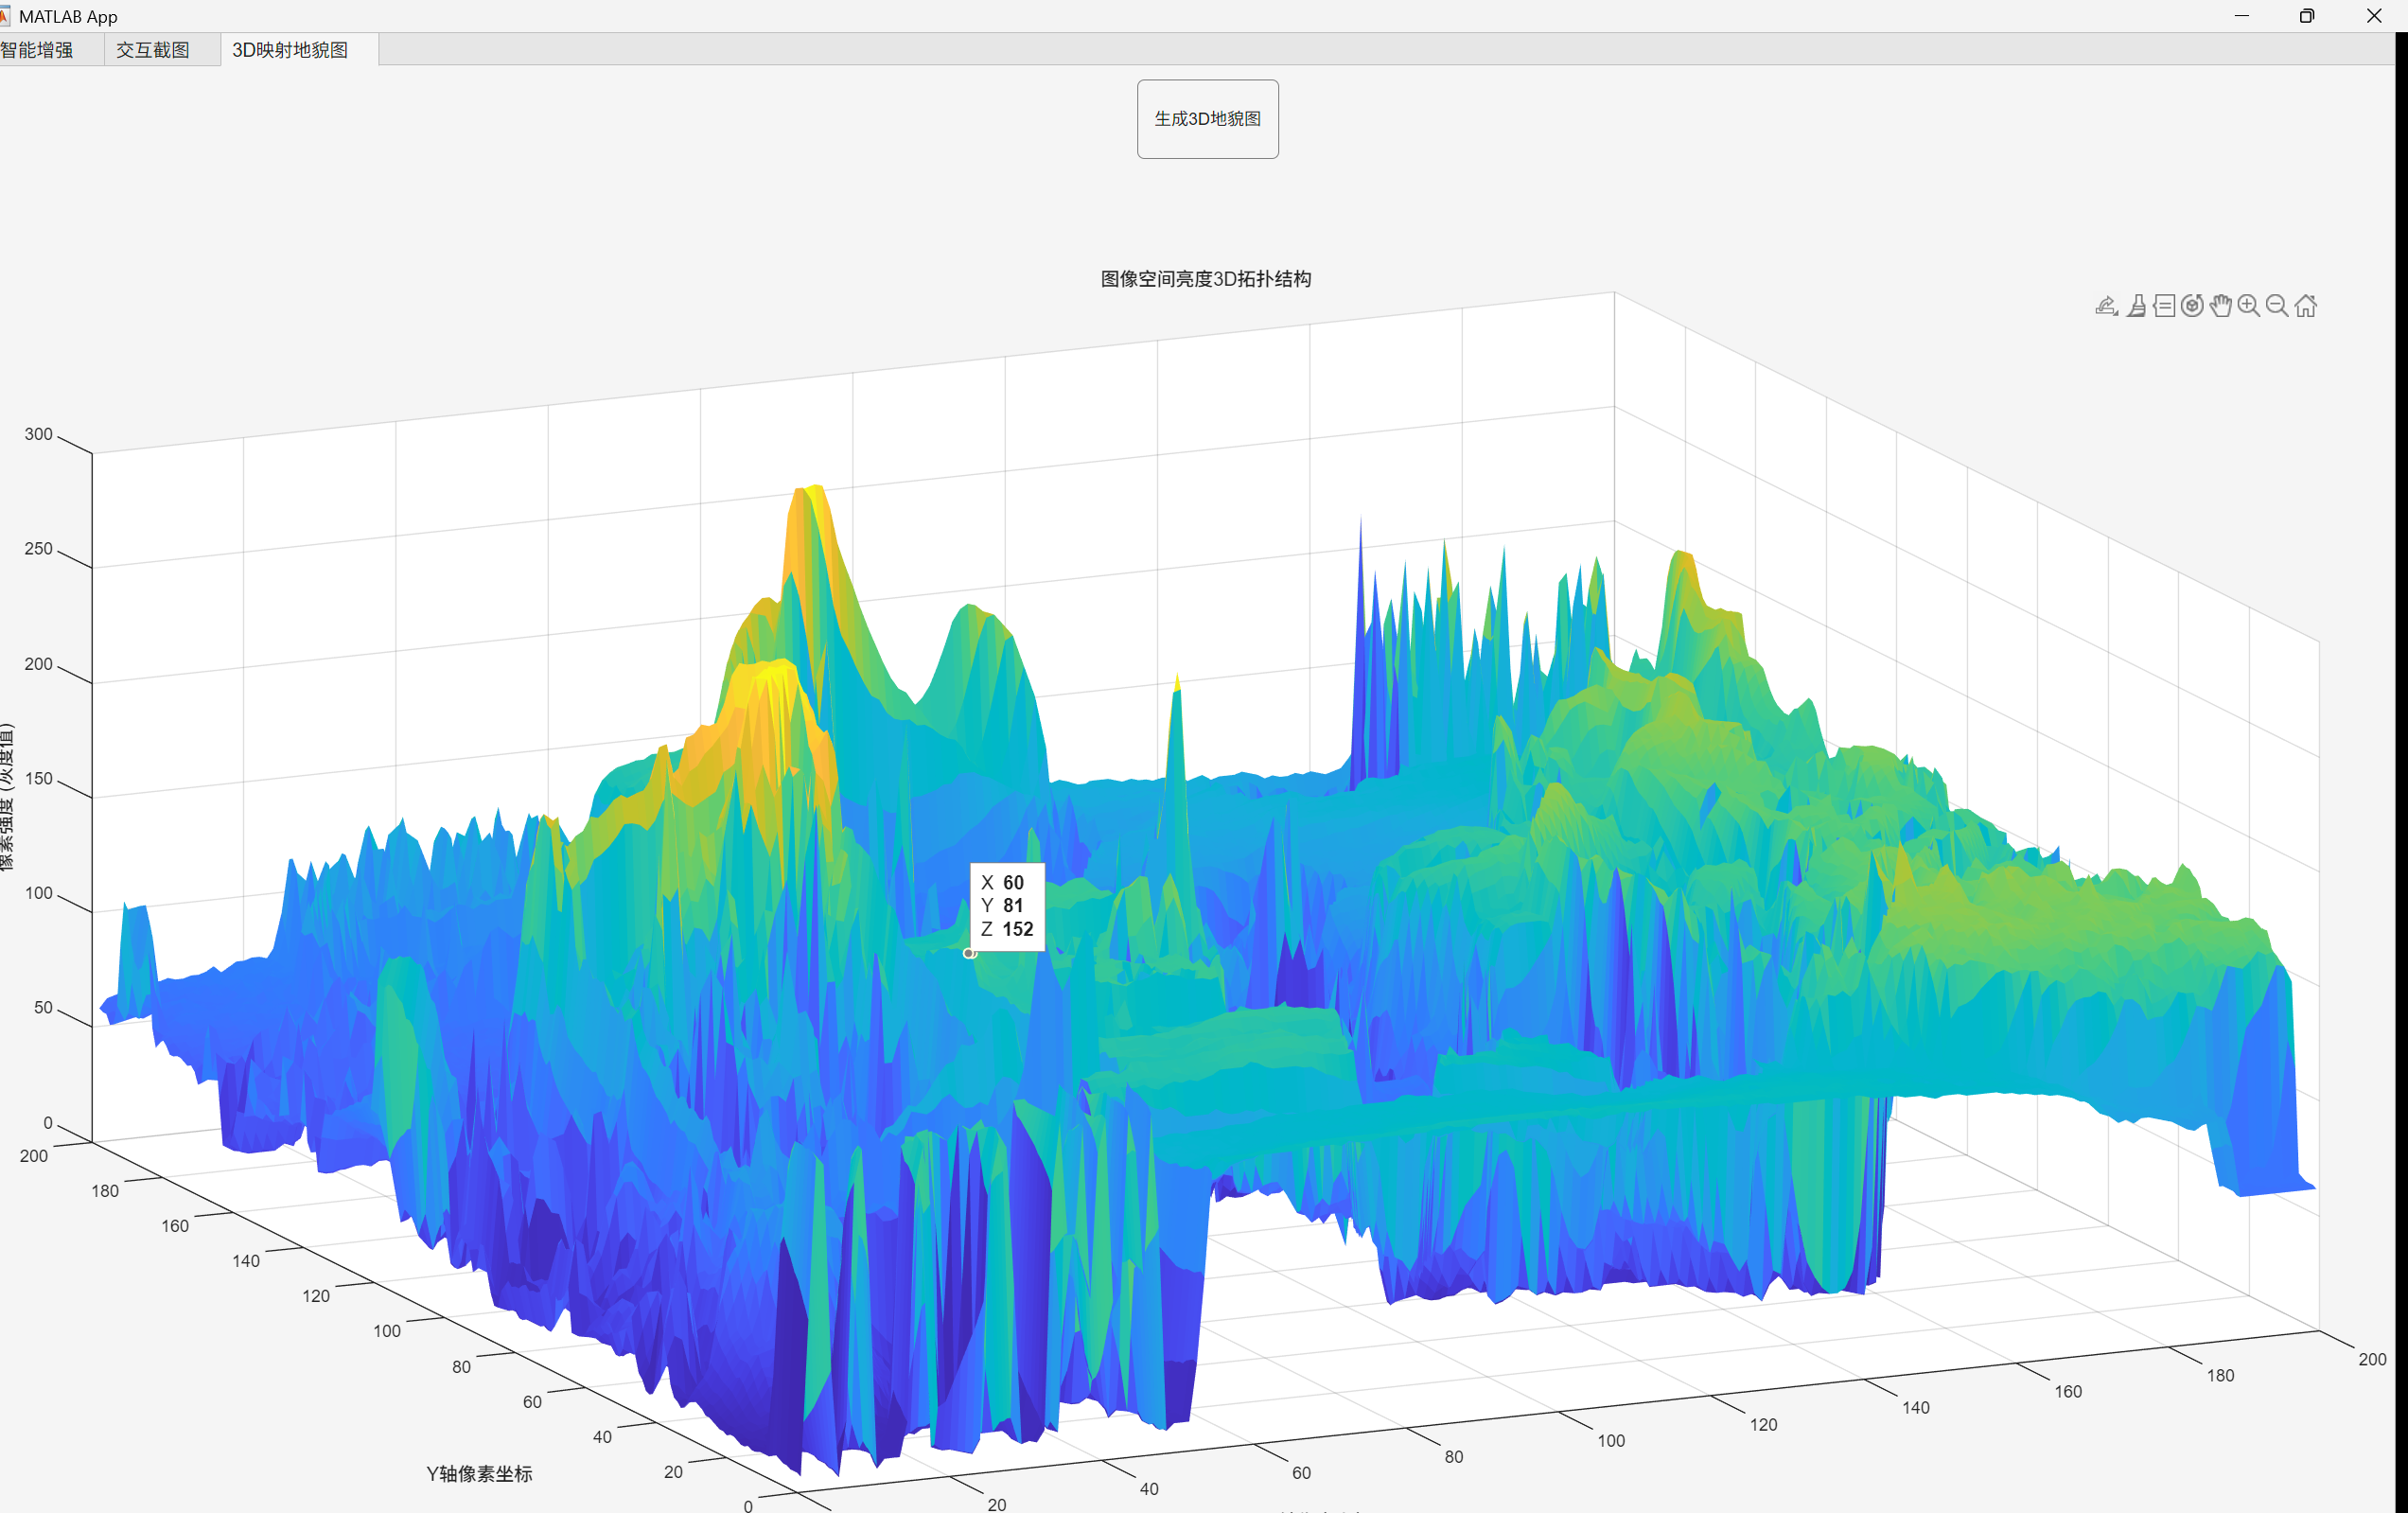
\includegraphics[width=0.8\textwidth]{view_3d.png}
    \caption{3D地貌图旋转展示}
    \label{fig:3d}
\end{figure}

\section{调试过程与遇到的问题及解决办法}
在开发这个 App 的过程中，我遇到了几个具体交互和编译逻辑问题，通过查阅文档和学习b站资料解决：

\begin{enumerate}
    \item \textbf{手绘框选时图片移位问题：}
    在编写第二个选项卡时，我发现用鼠标拖动红框时，背景图片经常会跟着一起漂移，导致裁剪错位。经过排查，发现这是由于 MATLAB 画板默认开启了平移手势。
    \\ \textbf{解决办法：} 在画框前加入 \texttt{disableDefaultInteractivity(app.UIAxes\_SegMain)} 语句，锁死背景图，彻底解决了画框与拖图的手势冲突。
    
    \item \textbf{双击空白处或关闭时报错问题：}
    在测试 ROI 裁剪时，如果鼠标不小心在画板上双击或者直接关闭窗口，后台命令行会弹出一堆坐标未定义的报错。
    \\ \textbf{解决办法：} 整个框选代码包在 \texttt{try-catch} 块中。这样即使操作中途被强行中断，程序也会退出。
    
    \item \textbf{添加私有函数时按钮变灰问题：}
    在编写后台实时截图函数时，我发现 Code View 顶部的“添加函数”按钮一直是灰色的，无法点击。
    \\ \textbf{解决办法：} 查阅手册后发现是因为鼠标光标停留位置不对导致系统丢失了焦点。我直接通过手动编写 \texttt{methods (Access = private)} 声明代码块，直接写进底层的类定义中。
\end{enumerate}

\begin{figure}[H]
    \centering
    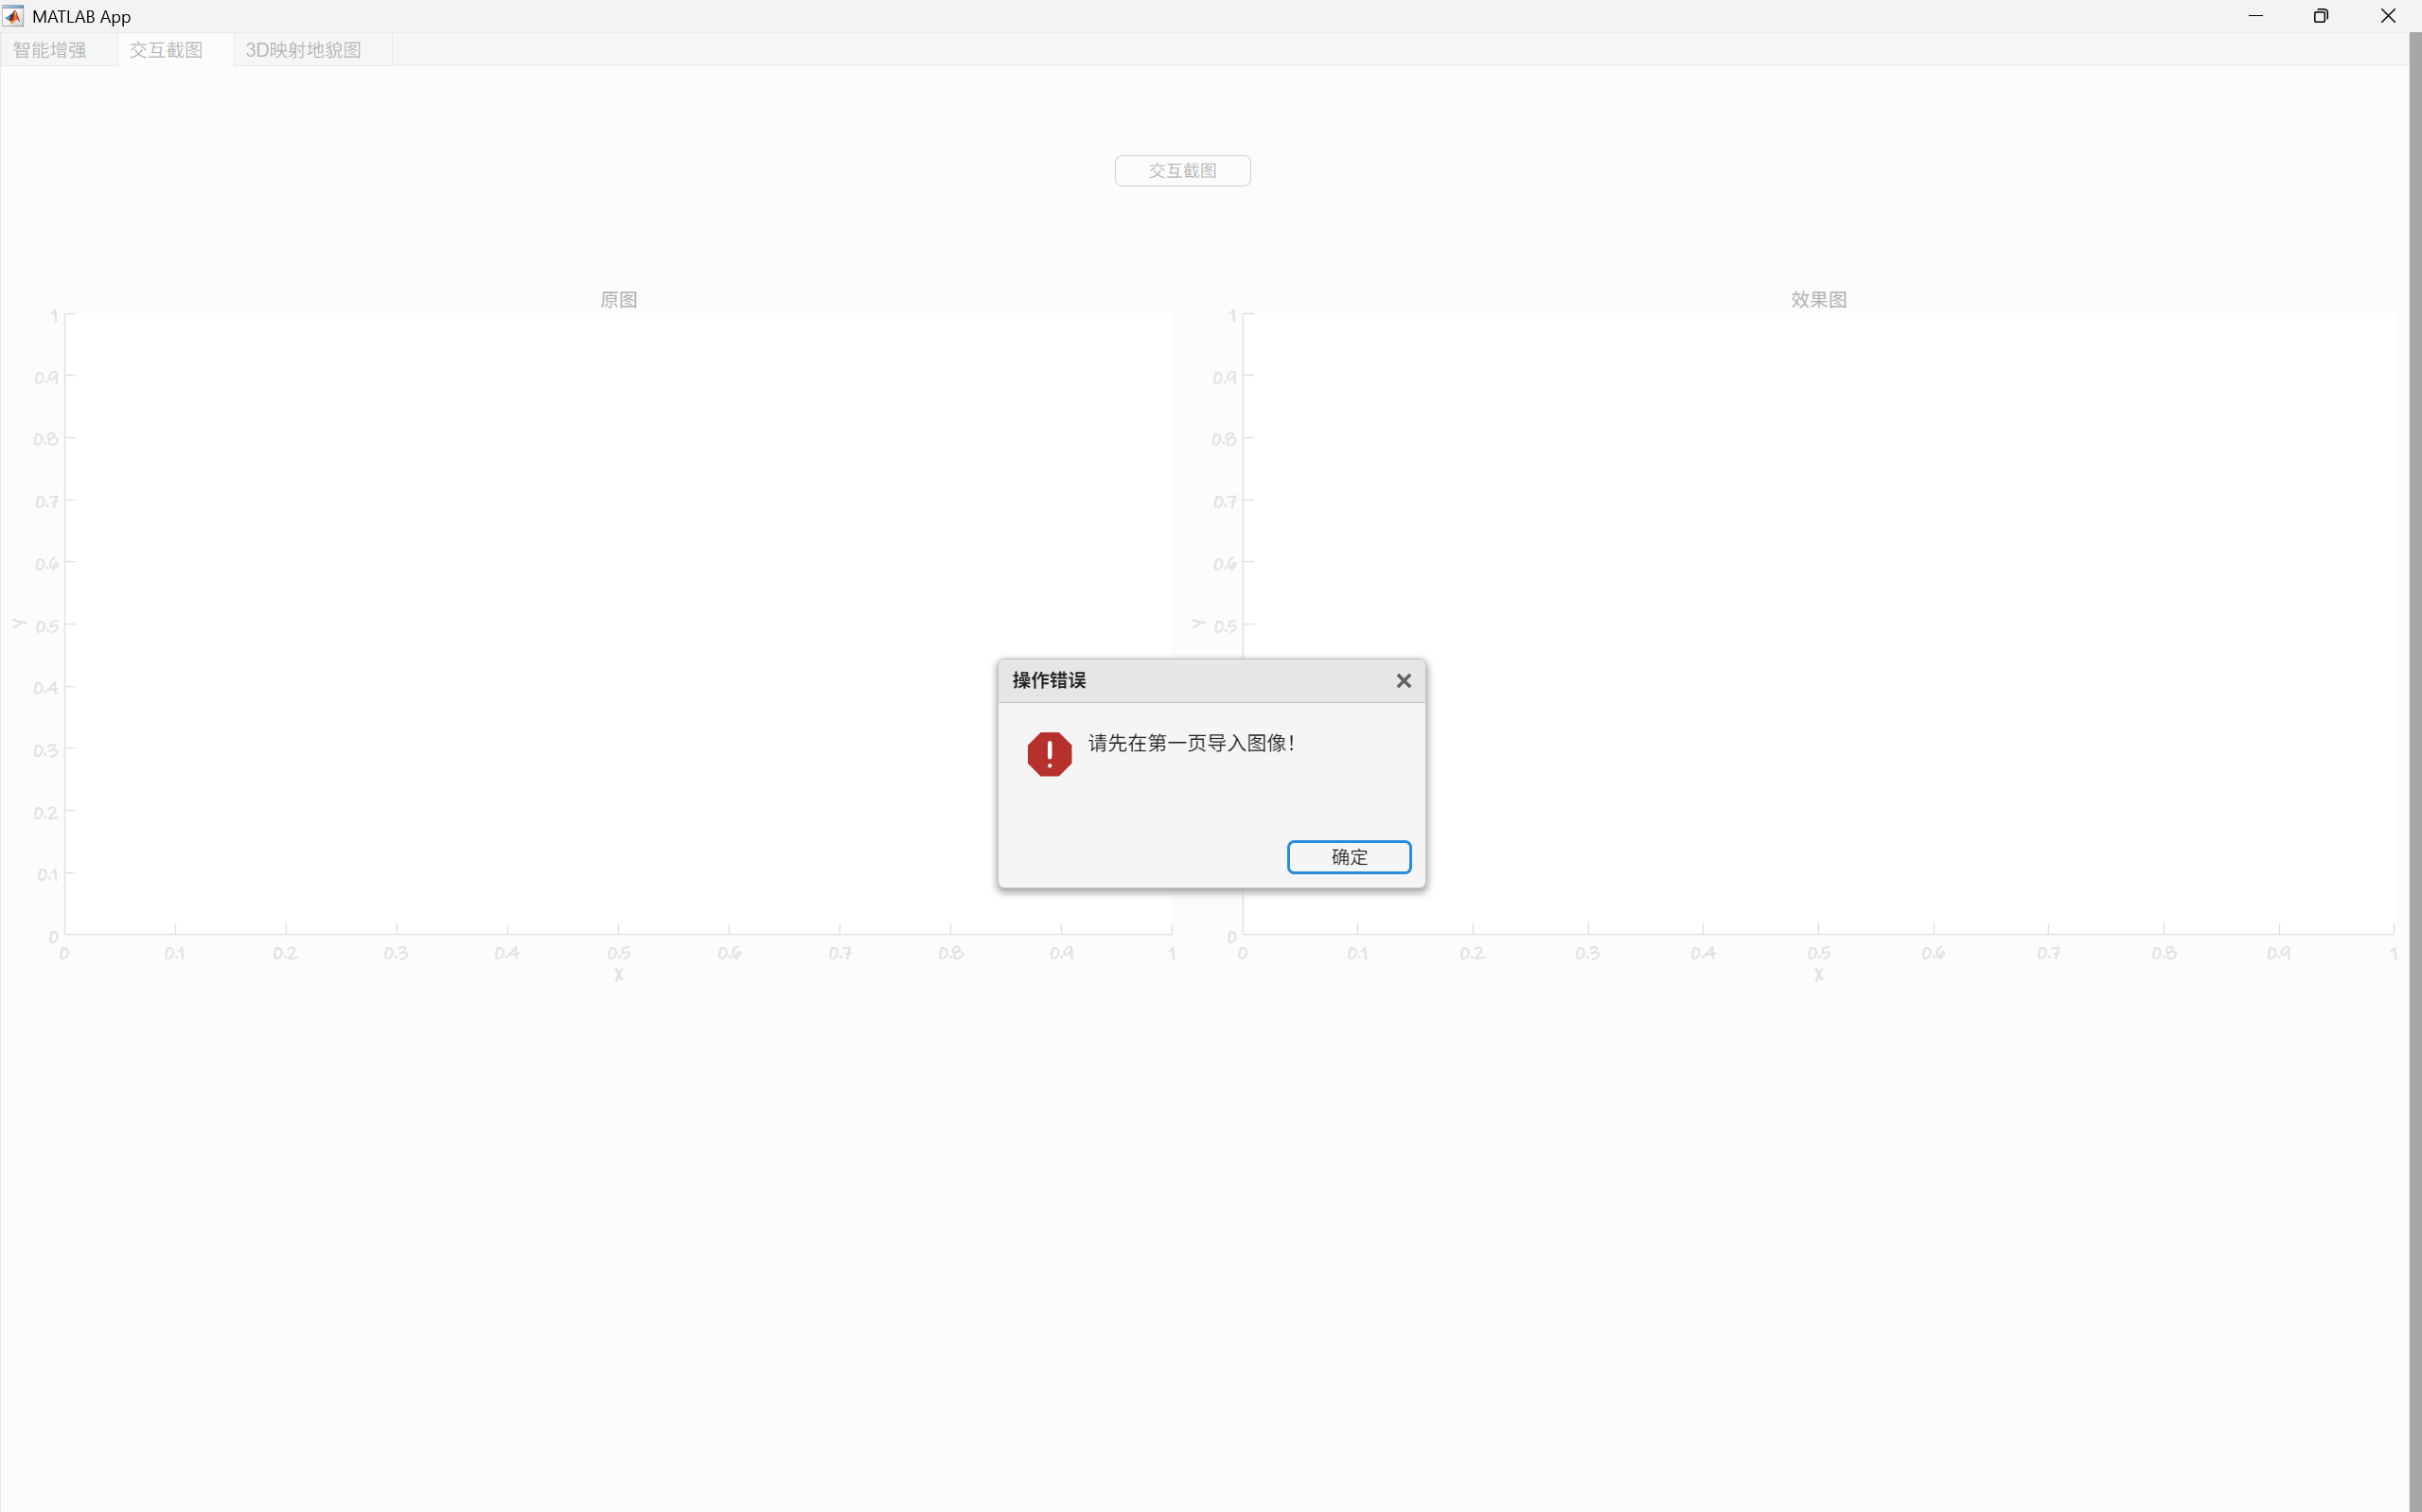
\includegraphics[width=0.6\textwidth]{alert2.png}
    \caption{系统异常防御与提示弹窗}
    \label{fig:alert2}
\end{figure}

\section{总结与设计收获}
这次基于 MATLAB App Designer 的课程设计，不仅让我巩固了课本上关于数字信号处理和矩阵映射的算法知识，更重要的是锻炼了我的软件工程实践能力。

在设计过程中，我理解了如何通过“私有属性”管理数据流，如何利用“事件监听器”设计出响应快速的交互界面。最后，我成功将项目打包发布为 \texttt{.mltbx} 格式的安装包，完成了从界面排版代码编写到打包发布的完整流程。这为我后续本科eecs路打下了matlab软件基础。

\end{document}